\documentclass[18pt,xcolor=table]{beamer}
\usepackage{amsmath, amssymb, amsthm, mathtools}
\usepackage{graphicx}
\usepackage{cancel}
\usepackage{color}
\usepackage{caption}
\usepackage{subcaption}
%\usepackage{subfigure}
\usepackage{pgf,tikz}
\usetikzlibrary{arrows}

\captionsetup{compatibility=false}

\newcommand{\bs}[1]{\boldsymbol{#1}}
\newcommand{\norm}[1]{\left\| #1 \right\|}
\newcommand{\snorm}[1]{\left| #1 \right|}
\newcommand{\LRp}[1]{\left( #1 \right)}
\newcommand{\LRs}[1]{\left[ #1 \right]}
\newcommand{\LRc}[1]{\left\{ #1 \right\}}
\newcommand{\LRa}[1]{\left\langle #1 \right\rangle}
\newcommand{\LRb}[1]{\left| #1 \right|}
\newcommand{\Grad}{\ensuremath{\nabla}}
\newcommand{\Gradxt}{\ensuremath{\nabla_{xt}}}
\newcommand{\Div}{\ensuremath{\nabla\cdot}}
\newcommand{\Divxt}{\ensuremath{\nabla_{xt}\cdot}}
\newcommand{\Curl}{\ensuremath{\nabla\times}}
\newcommand{\bfH}{\mbox{\boldmath $H$}}
\newcommand{\bfsigma}{\boldsymbol\sigma}
\newcommand{\bfvarsigma}{\boldsymbol\varsigma}
\newcommand{\bftau}{\boldsymbol\tau}
\newcommand{\bfbeta}{\boldsymbol\beta}
\newcommand{\bflambda}{\boldsymbol\lambda}
\newcommand{\bfpsi}{\boldsymbol\psi}
\newcommand{\bfu}{\boldsymbol u}
\newcommand{\bfv}{\boldsymbol v}
\newcommand{\bfV}{\boldsymbol V}
\newcommand{\bfZ}{\boldsymbol Z}
\newcommand{\bfz}{\boldsymbol z}
\newcommand{\bfW}{\boldsymbol W}
\newcommand{\bfw}{\boldsymbol w}
\newcommand{\bfm}{\boldsymbol m}
\newcommand{\bfM}{\boldsymbol M}
\newcommand{\bbM}{\mathbb{M}}
\newcommand{\bfq}{\boldsymbol q}
\newcommand{\bfU}{\boldsymbol U}
\newcommand{\bfS}{\boldsymbol S}
\newcommand{\bbS}{\mathbb{S}}
\newcommand{\bbD}{\mathbb{D}}
\newcommand{\bfK}{\boldsymbol K}
\newcommand{\bbK}{\mathbb{K}}
\newcommand{\bfn}{\boldsymbol n}
\newcommand{\bff}{\boldsymbol f}
\newcommand{\bfF}{\boldsymbol F}
\newcommand{\bbF}{\mathbb{F}}
\newcommand{\bfg}{\boldsymbol g}
\newcommand{\bfG}{\boldsymbol G}
\newcommand{\bfC}{\boldsymbol C}
\newcommand{\bft}{\boldsymbol t}
\newcommand{\bfT}{\boldsymbol T}
\newcommand{\bfI}{\boldsymbol I}
\newcommand{\bbI}{\mathbb{I}}
\newcommand{\bfx}{\boldsymbol x}
\newcommand{\uh}{\widehat{u}}
\newcommand{\fnh}{\widehat{f}_n}
\newcommand{\LQ}{L^2\LRp{Q}}
\newcommand{\LK}{L^2\LRp{K}}
\newcommand{\LVecK}{\mathbf{L}^2\LRp{K}}
\newcommand{\LVecQ}{\mathbf{L}^2\LRp{Q}}
\newcommand{\HdivK}{\bfH(\text{div},K)}
\newcommand{\HdivOmega}{\bfH(\text{div},\Omega)}
% \newcommand{\HdivOmegaLT}{\bfH(\text{div},\Omega)\times L^2([0,T])}
\newcommand{\HdivQ}{\bfH(\text{div}_{xt},Q)}
\newcommand{\HOneK}{H^{1}(K)}
\newcommand{\HOneVecK}{\bfH^{1}(K)}
\newcommand{\HOneQ}{H^{1}(Q)}
\newcommand{\HOneOmegah}{H^{-1}(\Omega_h)}
\newcommand{\HdivOmegah}{\bfH(\text{div},\Omega_h)}
\newcommand{\vdeltau}{v_{\delta\bs u_h}}
\newcommand{\taudeltau}{\bftau_{\delta\bs u_h}}
\newcommand{\ip}[1]{\left\langle #1 \right\rangle}
\newcommand{\pd}[2]{\frac{\partial#1}{\partial#2}}
\newcommand{\pt}[1]{\frac{\partial#1}{\partial t}}
\newcommand{\ppd}[2]{\frac{\partial^2#1}{\partial#2^2}}
\newcommand{\pdd}[3]{\frac{\partial^2#1}{\partial#2\partial#3}}
\newcommand{\der}[2]{\frac{\mathrm{d}#1}{\mathrm{d}#2}}
\newcommand{\Oh}{\Omega_h}
\newcommand{\jump}[1] {\ensuremath{\LRs{\![#1]\!}}}
\newcommand{\Gh}{\Gamma_h}
\newcommand{\mcU}{\mathcal{U}}
\newcommand{\mcUh}{\hat{\mathcal{U}}}
\newcommand{\LOmega}{L^2\LRp{\Omega_h}}

\newcommand{\eqnref}[1]{\eqref{eq:#1}}

\DeclareMathOperator*{\argmin}{arg\,min}
\DeclareMathOperator*{\trace}{tr}

\def\arrtwo#1#2#3#4{\left[
\begin{array}{cc}
#1\; & #2\\
#3\; & #4\\
\end{array}
\right]}
\def\arrthree#1#2#3#4#5#6#7#8#9{\left[
\begin{array}{ccc}
#1\; & #2\; & #3\\
#4\; & #5\; & #6\\
#7\; & #8\; & #9\\
\end{array}
\right]}
\def\arrthreeone#1#2#3{\left[
\begin{array}{ccc}
#1\; & #2\; & #3\\
\end{array}
\right]}
\def\vecttwo#1#2{\left(
\begin{array}{c}
#1\\
#2\\
\end{array}
\right)}
\def\svecttwo#1#2{\left[
\begin{array}{c}
#1\\
#2\\
\end{array}
\right]}
\def\vectthree#1#2#3{\left(
\begin{array}{c}
#1\\
#2\\
#3\\
\end{array}
\right)}
\def\svectthree#1#2#3{\left[
\begin{array}{c}
#1\\
#2\\
#3\\
\end{array}
\right]}

\renewcommand{\arraystretch}{1.2}

\def\etal{{\it et al.~}}

\graphicspath{{./figs/}}

\usepackage{bbm}
\usepackage{textpos}
\usepackage{pgf,tikz}
\usepackage{graphicx}
\usepackage{forloop}

\definecolor{utorange}{RGB}{203,96,21}
\definecolor{utblack}{RGB}{99,102,106}
\definecolor{utbrown}{RGB}{110,98,89}
\definecolor{utsecbrown}{RGB}{217,200,158}
\definecolor{utsecgreen}{RGB}{208,222,187}
\definecolor{utsecblue}{RGB}{127,169,174}

\mode<presentation>
{
  % \usetheme{Pittsburgh}
  \usetheme{Boadilla}
  \usefonttheme[onlymath]{serif}

  \setbeamercovered{invisible}
  \setbeamertemplate{navigation symbols}{}

  % Color Theme
    \setbeamercolor{normal text}{bg=white,fg=utblack}
  \setbeamercolor{structure}{fg=utorange}

  \setbeamercolor{alerted text}{fg=red!85!black}

  \setbeamercolor{item projected}{use=item,fg=black,bg=item.fg!35}

  \setbeamercolor*{palette primary}{use=structure,fg=white, bg=utorange}
  \setbeamercolor*{palette secondary}{use=structure,bg=utsecbrown}
  \setbeamercolor*{palette tertiary}{use=structure,bg=utsecgreen}
  \setbeamercolor*{palette quaternary}{use=structure,fg=structure.fg,bg=utsecblue}

  % \setbeamercolor*{frametitle}{use=structure,fg=utorange, bg=utsecbrown}
  \setbeamercolor*{framesubtitle}{fg=utbrown}

  \setbeamercolor*{block title}{parent=structure,fg=black,bg=utsecgreen}
  \setbeamercolor*{block body}{fg=black,bg=utblack!10}
  \setbeamercolor*{block title alerted}{parent=alerted text,bg=black!15}
  \setbeamercolor*{block title example}{parent=example text,bg=black!15}

  \setbeamerfont{framesubtitle}{size=\small}
}

% \usepackage[orientation=landscape,size=custom,width=16,height=9.75,scale=0.5,debug]{beamerposter}
% \usepackage[orientation=landscape,size=custom,width=16,height=9,scale=0.5,debug]{beamerposter}


\makeatletter
\setbeamertemplate{footline}
{
  \leavevmode%
    \hbox{%
      \begin{beamercolorbox}[wd=.333333\paperwidth,ht=2.25ex,dp=1ex,center]{author in head/foot}%
        \usebeamerfont{author in head/foot}\insertshortauthor%~~\beamer@ifempty{\insertshortinstitute}{}{(\insertshortinstitute)}
      \end{beamercolorbox}%
        \begin{beamercolorbox}[wd=.333333\paperwidth,ht=2.25ex,dp=1ex,center]{title in head/foot}%
        \usebeamerfont{title in head/foot}\insertshorttitle
        \end{beamercolorbox}%
        \begin{beamercolorbox}[wd=.333333\paperwidth,ht=2.25ex,dp=1ex,right]{date in head/foot}%
        \usebeamerfont{date in head/foot}\insertshortdate{}\hspace*{2em}
        \insertframenumber{} / \inserttotalframenumber\hspace*{2ex}
      \end{beamercolorbox}}%
        \vskip0pt%
}
\makeatother

\usepackage{kerkis}
\usepackage[T1]{fontenc}
\usepackage[protrusion=true,expansion=true]{microtype}
\usepackage{amsmath}


\renewcommand*{\thefootnote}{\fnsymbol{footnote}}


\pgfdeclareimage[height=1.2cm]{utbig}{logos/UTWordmark}
\pgfdeclareimage[height=0.6cm]{ut}{logos/UTWordmark}
% \pgfdeclareimage[height=10.0cm]{utbig}{logos/ICES-wordmark-teal.pdf}
% \pgfdeclareimage[height=0.6cm]{ut}{logos/ICES-wordmark-teal.pdf}
% \pgfdeclareimage[height=1.5cm]{iceslogo}{logos/ICES-wordmark-teal.png}
% \pgfdeclareimage[height=1.0cm]{scsmall}{logos/SC12}

\title[Space-Time DPG for Parallel CFD]{Space-Time DPG:\\ Designing a Method for Parallel CFD}
% \subtitle{If you have one}
\author[Truman E. Ellis]{ \underline{Truman~Ellis} \\
Leszek Demkowicz, Nathan Roberts, Jesse Chan, Robert Moser
}

% \institute{Institute for Computational Engineering \& Sciences\\ \mbox{}  \\  \pgfuseimage{utbig} }
\institute{
\pgfuseimage{utbig}
\\ \vspace{2ex}

\includegraphics[trim=3.0in 7.2in 1.5in 4.0in,width=0.3\linewidth]{logos/ICES-wordmark-teal.pdf}
}
\date[Finite Element Rodeo 2014]%{\pgfuseimage{iceslogo} }

\begin{document}

\tikzstyle{block} = [rectangle, draw, rounded corners, shade, top color=white, text width=5em,
  bottom color=blue!50!black!20, draw=blue!40!black!60, very thick, text centered, minimum height=4em]
  \tikzstyle{line} = [draw, -latex']
  \tikzstyle{cloud} = [draw, ellipse,top color=white, bottom color=red!20, node distance=2cm, minimum height=2em]


  \beamertemplateballitem
  %\beamertemplatetransparentcoveredhigh

  \frame{\titlepage}

  \addtobeamertemplate{frametitle}{}{%
      \begin{textblock*}{100mm}(0.87\textwidth,-0.75cm)
    \pgfuseimage{ut}
    \end{textblock*}
  }


\section{Introduction}

% ------------------------------------------------------------
\begin{frame}[t]
\frametitle{Motivation}
\framesubtitle{DPG Summary}  %% needed for proper positioning of the logo ...
Overview of Features
\begin{itemize}
\item Robust for singularly perturbed problems
\item Stable in the preasymptotic regime
\item Designed for adaptive mesh refinement
\end{itemize}
\bigskip

DPG is a minimum residual method:
\[
u_{h} = \underset{w_{h} \in U_{h}} \argmin \,\, \frac{1}{2}
\norm{Bw_{h}-l}_{V'}^{2}
\]
\vspace{-1em}
\[
\scalebox{1.8}{\ensuremath{\Updownarrow}}
\]
\vspace{-1em}
\[
b(u_h,R_V^{-1}B\delta u_h)
=l(R_V^{-1}B\delta u_h)
\quad\forall\delta u_h\in U_h
\]
\vspace{0ex}

where $v_{\delta u_h}:=R_V^{-1}B\delta u_h$ are the
\textcolor{utblack}{\textbf{optimal test functions}}.

\end{frame}

%   /$$   /$$                       /$$    
%  | $$  | $$                      | $$    
%  | $$  | $$  /$$$$$$   /$$$$$$  /$$$$$$  
%  | $$$$$$$$ /$$__  $$ |____  $$|_  $$_/  
%  | $$__  $$| $$$$$$$$  /$$$$$$$  | $$    
%  | $$  | $$| $$_____/ /$$__  $$  | $$ /$$
%  | $$  | $$|  $$$$$$$|  $$$$$$$  |  $$$$/
%  |__/  |__/ \_______/ \_______/   \___/  
%                                          
%                                          
%  
\section{Heat Equation}

% ------------------------------------------------------------
\begin{frame}[t]
\frametitle{Heat Equation}
\framesubtitle{Simplest Nontrivial Space-Time Problem}  %% needed for proper positioning of the logo ...

Equation is elliptic in space, but hyperbolic in time.
\begin{equation*}
  \frac{\partial u}{\partial t}-\epsilon\Delta u=f
\end{equation*}

This is really just a composite of Fourier's law and conservation of energy.
\begin{equation*}
\begin{aligned}
\bfsigma-\epsilon\Grad u&=0\\
\frac{\partial u}{\partial t}-\Div\bfsigma&=f
\end{aligned}
\end{equation*}

We can rewrite this in terms of a space-time divergence.
\begin{equation*}
\begin{aligned}
\frac{1}{\epsilon}\bfsigma-\Grad u&=0\\
\Divxt\vecttwo{-\bfsigma}{u}&=f
\end{aligned}
\end{equation*}

\end{frame}

% ------------------------------------------------------------
\begin{frame}[t]
\frametitle{Heat Equation}
\framesubtitle{DPG Formulation}  %% needed for proper positioning of the logo ...
\vspace{-2ex}
Multiply by test function and integrate by parts over space-time element K.
\begin{equation*}
\begin{aligned}
\LRp{\frac{1}{\epsilon}\bfsigma,\bftau}+\LRp{u,\Div\bftau}-\LRa{\hat u,\bftau\cdot\bfn_x}&=0\\
-\LRp{\vecttwo{-\bfsigma}{u},\Gradxt v}+\LRa{\hat t,v}&=f
\end{aligned}
\end{equation*}
\begin{columns}[t] % contents are top vertically aligned
\begin{column}[T]{0.4\textwidth} % each column can also be its own environment
where
\begin{align*}
\hat u&:=\trace(u)\\
\hat t&:=\trace(-\bfsigma)\cdot\bfn_x+\trace(u)\cdot n_t
\end{align*}
\vspace{-4ex}
\begin{itemize}
  \item Trace $\hat u$ defined on spatial boundaries
  \item Flux $\hat t$ defined on all boundaries
\end{itemize}
\end{column}
\begin{column}[T]{0.6\textwidth} % alternative top-align that's better for graphics
\vspace{-2ex}
\begin{block}{Support of Trace Variables}
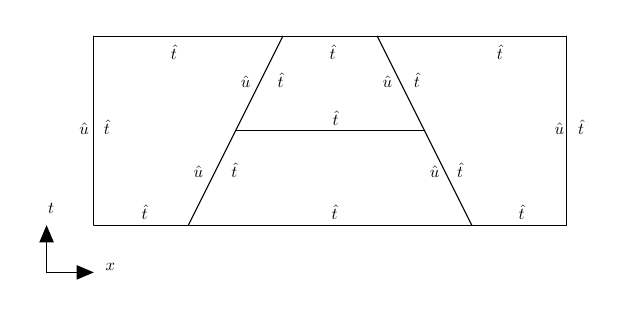
\begin{tikzpicture}[line cap=round,line join=round,>=triangle 45,x=2.0cm,y=2.0cm, scale=0.6, every node/.style={scale=0.6}]
\clip(-0.7,-0.6) rectangle (5.27,2.09);
\draw (0,2)-- (0,0);
\draw (0,0)-- (1,0);
\draw (1,0)-- (4,0);
\draw (4,0)-- (5,0);
\draw (5,0)-- (5,2);
\draw (5,2)-- (3,2);
\draw (3,2)-- (2,2);
\draw (2,2)-- (0,2);
\draw (1,0)-- (1.5,1);
\draw (1.5,1)-- (2,2);
\draw (1.5,1)-- (3.5,1);
\draw (3,2)-- (3.5,1);
\draw (3.5,1)-- (4,0);
\draw (-0.21,0.9) node[anchor=south west] {$\hat u$};
\draw (4.82,0.9) node[anchor=south west] {$\hat u$};
\draw (3.5,0.45) node[anchor=south west] {$\hat u$};
\draw (1.0,0.45) node[anchor=south west] {$\hat u$};
\draw (1.5,1.4) node[anchor=south west] {$\hat u$};
\draw (3.0,1.4) node[anchor=south west] {$\hat u$};
\draw (0.05,0.9) node[anchor=south west] {$\hat t$};
\draw (1.40,0.45) node[anchor=south west] {$\hat t$};
\draw (3.79,0.45) node[anchor=south west] {$\hat t$};
\draw (2.47,1.0) node[anchor=south west] {$\hat t$};
\draw (3.33,1.4) node[anchor=south west] {$\hat t$};
\draw (1.89,1.4) node[anchor=south west] {$\hat t$};
\draw (5.07,0.9) node[anchor=south west] {$\hat t$};
\draw (4.44,0.0) node[anchor=south west] {$\hat t$};
\draw (2.46,0.0) node[anchor=south west] {$\hat t$};
\draw (0.45,0.0) node[anchor=south west] {$\hat t$};
\draw (2.44,1.7) node[anchor=south west] {$\hat t$};
\draw (0.76,1.7) node[anchor=south west] {$\hat t$};
\draw (4.21,1.7) node[anchor=south west] {$\hat t$};
\draw [->] (-0.5,-0.5) -- (-0.5,0);
\draw [->] (-0.5,-0.5) -- (0,-0.5);
\draw (-0.54,0.29) node[anchor=north west] {$t$};
\draw (0.07,-0.35) node[anchor=north west] {$x$};
\end{tikzpicture}
\end{block}
\end{column}
\end{columns}


\end{frame}

% ------------------------------------------------------------
\begin{frame}[t]
\frametitle{Heat equation}
\framesubtitle{Pulsed Source Problem}  %% needed for proper positioning of the logo ...
\vspace{-3ex}
\begin{columns}[t] % contents are top vertically aligned
\begin{column}[T]{0.3\textwidth} % each column can also be its own environment
\end{column}
\begin{column}[T]{0.7\textwidth} % each column can also be its own environment
\begin{figure}[ht]
\centering
\begin{subfigure}[t]{0.45\textwidth}
\centering
\includegraphics[height=0.8\textwidth]{SpaceTimeHeat/PulseSource/u.png}
\\$u$\\\vspace{1ex}
\end{subfigure}
\begin{subfigure}[t]{0.45\textwidth}
\centering
\includegraphics[height=0.8\textwidth]{SpaceTimeHeat/PulseSource/sigma.png}
\\$\sigma$\\\vspace{1ex}
\end{subfigure}
\begin{subfigure}[t]{0.45\textwidth}
\centering
\includegraphics[height=0.8\textwidth]{SpaceTimeHeat/PulseSource/uhat.png}
\\$\hat u$
\end{subfigure}
\begin{subfigure}[t]{0.45\textwidth}
\centering
\includegraphics[height=0.8\textwidth]{SpaceTimeHeat/PulseSource/fhat.png}
\\$\hat t$
\end{subfigure}
% \caption{Pulsed space-time heat problem after 4 refinements}
\end{figure}
\end{column}
\end{columns}
\end{frame}

%    /$$$$$$                                                                            /$$ /$$       /$$          
%   /$$__  $$                                                                          |__/| $$      | $$          
%  | $$  \__/  /$$$$$$  /$$$$$$/$$$$   /$$$$$$   /$$$$$$   /$$$$$$   /$$$$$$$  /$$$$$$$ /$$| $$$$$$$ | $$  /$$$$$$ 
%  | $$       /$$__  $$| $$_  $$_  $$ /$$__  $$ /$$__  $$ /$$__  $$ /$$_____/ /$$_____/| $$| $$__  $$| $$ /$$__  $$
%  | $$      | $$  \ $$| $$ \ $$ \ $$| $$  \ $$| $$  \__/| $$$$$$$$|  $$$$$$ |  $$$$$$ | $$| $$  \ $$| $$| $$$$$$$$
%  | $$    $$| $$  | $$| $$ | $$ | $$| $$  | $$| $$      | $$_____/ \____  $$ \____  $$| $$| $$  | $$| $$| $$_____/
%  |  $$$$$$/|  $$$$$$/| $$ | $$ | $$| $$$$$$$/| $$      |  $$$$$$$ /$$$$$$$/ /$$$$$$$/| $$| $$$$$$$/| $$|  $$$$$$$
%   \______/  \______/ |__/ |__/ |__/| $$____/ |__/       \_______/|_______/ |_______/ |__/|_______/ |__/ \_______/
%                                    | $$                                                                          
%                                    | $$                                                                          
%                                    |__/    
\section{Compressible Navier-Stokes}

% ------------------------------------------------------------
\begin{frame}[t]
\frametitle{Compressible Navier-Stokes}
\framesubtitle{Strong Form}  %% needed for proper positioning of the logo ...
The compressible Navier-Stokes equations are
\begin{align*}
\frac{\partial}{\partial t}\svectthree{\rho}{\rho\bfu}{\rho e_0}
+\Div\svectthree{\rho\bfu}{\rho\bfu\otimes\bfu+p\bfI-\mathbb{D}}{\rho\bfu e_0+\bfu p+\bfq-\bfu\cdot\mathbb{D}}
%TODO: Possible error above. cfd-online seems to have T^T
=\svectthree{f_c}{\bff_m}{f_e}\,,
\end{align*}
where
\begin{equation*}
  \mathbb{D}=2\mu\bfS^*=2\mu\LRs{\frac{1}{2}\LRp{\Grad\bfu+\LRp{\Grad\bfu}^T}-\frac{1}{3}\Div\bfu\bfI}\,,
\end{equation*}
\begin{equation*}
  \bfq=-C_p\frac{\mu}{Pr}\Grad T\,,
\end{equation*}
and (assuming an ideal gas EOS)
\[
p=\rho R T\,.
\]
\end{frame}

% ------------------------------------------------------------
\begin{frame}[t]
\frametitle{Compressible Navier-Stokes}
\framesubtitle{First Order Space-Time Form}  %% needed for proper positioning of the logo ...
Writing this in space-time in terms of $\rho$, $\bfu$, $T$, $\mathbb{D}$, and $\bfq$:
\begin{align*}
  \mathbb{D}-\mu\LRp{\Grad\bfu+\LRp{\Grad\bfu}^T}+\frac{2\mu}{3}\Div\bfu\bfI&=0\\
  \bfq+C_p\frac{\mu}{Pr}\Grad T&=0\\
  \Divxt\vecttwo{\rho\bfu}{\rho}&=f_c\\
  \Divxt\vecttwo{\rho\bfu\otimes\bfu+\rho RT\bfI-\mathbb{D}}{\rho\bfu}&=\bff_m\\
  \Divxt\vecttwo{\rho\bfu\LRp{C_v T+\frac{1}{2}\bfu\cdot\bfu}+\bfu\rho RT+\bfq-\bfu\cdot\mathbb{D}}{\rho\LRp{C_v T+\frac{1}{2}\bfu\cdot\bfu}}&=f_e\,.
\end{align*}
\end{frame}


% ------------------------------------------------------------
\begin{frame}[t]
\frametitle{Compressible Navier-Stokes}
\framesubtitle{DPG Formulation}  %% needed for proper positioning of the logo ...
Multiplying by test functions and integrating by parts:
% \scalebox{0.9}{
{
\small
\begin{align*}
  \LRp{\mathbb{D},\mathbb{S}}+\LRp{2\mu\bfu,\Div\mathbb{S}}-\LRp{\frac{2\mu}{3}\bfu,\Grad\trace{\mathbb{S}}}
  -\LRa{2\mu\hat\bfu,\mathbb{S}\bfn_x}+\LRa{\frac{2\mu}{3}\hat\bfu,\mathbb{S}\bfn_x}&=0\\
  \LRp{\bfq,\bftau}-\LRp{C_p\frac{\mu}{Pr}T,\Div\bftau}+\LRa{C_p\frac{\mu}{Pr}\hat T,\tau_n}&=0\\
  -\LRp{\vecttwo{\rho\bfu}{\rho},\Gradxt v_c}+\LRa{\hat t_c,v_c}&=\LRp{f_c,v_c}\\
  -\LRp{\vecttwo{\rho\bfu\otimes\bfu+\rho RT\bfI-\mathbb{D}}{\rho\bfu},\Gradxt\bfv_m}+\LRa{\hat\bft_m,\bfv_m}&=\LRp{\bff_m,\bfv_m}\\
  -\LRp{\vecttwo{\rho\bfu\LRp{C_v T+\frac{1}{2}\bfu\cdot\bfu}+\bfu\rho RT+\bfq-\bfu\cdot\mathbb{D}}{\rho\LRp{C_v T+\frac{1}{2}\bfu\cdot\bfu}},\Gradxt v_e}
  +\LRa{\hat t_e,v_e}&=\LRp{f_e,v_e}\,,
\end{align*}
}
% }
where $\hat u$ and $\hat T$ are spatial traces and $\hat t_c$, $\hat\bft_m$, and $\hat t_e$ are fluxes.
\end{frame}


% ------------------------------------------------------------
\begin{frame}[t]
\frametitle{Compressible Navier-Stokes}
\framesubtitle{Flux and Trace Variables}  %% needed for proper positioning of the logo ...
Spatial traces and fluxes are defined as follows:
\begin{equation*}
\begin{aligned}
\hat\bfu&=\trace(\bfu)\\
\hat T&=\trace(T)\\
\hat t_c&=\trace\LRp{\rho\bfu}\cdot\bfn_x
+\trace\LRp{\rho}n_t\\
\hat\bft_m&=\trace\LRp{\rho\bfu\otimes\bfu+\rho RT\bfI-\mathbb{D}}\cdot\bfn_x
+\trace\LRp{\rho\bfu} n_t\\
\hat t_e&=\trace\LRp{\rho\bfu\LRp{C_v T+\frac{1}{2}\bfu\cdot\bfu}+\bfu\rho RT+\bfq-\bfu\cdot\mathbb{D}}\cdot\bfn_x\\
&\quad+\trace\LRp{\rho\LRp{C_v T+\frac{1}{2}\bfu\cdot\bfu}}n_t\,.
\end{aligned}
\end{equation*}
\begin{block}{Linearization}
Fluxes, traces, and $\bfq$ are linear in the above bilinear form, but we need to linearize in $\rho$, $\bfu$, $T$, and $\mathbb{D}$ 
(Jacobian and residual not shown here).
\end{block}
\end{frame}


% % ------------------------------------------------------------
% \begin{frame}[t]
% \frametitle{Compressible Navier-Stokes}
% \framesubtitle{Linearization: Jacobian}  %% needed for proper positioning of the logo ...
% \end{frame}


% ------------------------------------------------------------
\begin{frame}[t]
\frametitle{Compressible Navier-Stokes}
\framesubtitle{Sod Shock Tube}  %% needed for proper positioning of the logo ...
% \foreach \n in {1,...,15}
% {
% \only<\n>
% {
% \vspace{-2ex}
% \begin{figure}[ht]
% \centering

% \begin{subfigure}[c]{0.45\textwidth}
% \centering
% \includegraphics[height=0.7\textwidth]{Sod1e-5/den\n.pdf}
% \end{subfigure}
% \begin{subfigure}[c]{0.45\textwidth}
% \centering
% \includegraphics[height=0.7\textwidth]{Sod1e-5/vel\n.pdf}
% \end{subfigure}
% \begin{subfigure}[c]{0.45\textwidth}
% \centering
% \includegraphics[height=0.7\textwidth]{Sod1e-5/pres\n.pdf}
% \end{subfigure}
% \begin{subfigure}[c]{0.45\textwidth}
% \centering
% \includegraphics[width=1\textwidth]{Sod1e-5/mesh\n.png}
% \end{subfigure}
% \end{figure}
% }
% }
\end{frame}

\end{document}
